
\begin{frame}
\frametitle{Introduction}
\framesubtitle{FGT Demo}


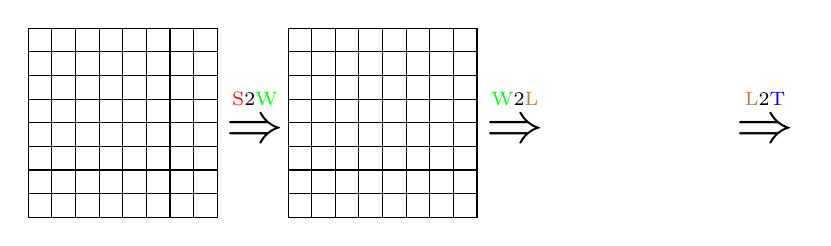
\begin{tikzpicture}[scale=1.2]

\draw (0,0) rectangle (2,2);

\foreach \ypos in {0.25, 0.5, ..., 1.75} {
 \draw (0, \ypos) -- (2, \ypos);
}

\foreach \xpos in {0.25, 0.5, ..., 1.75} {
 \draw (\xpos, 0) -- (\xpos, 2);
}

\draw (2.4, 0.9) node {\huge{$\Rightarrow$}};
\draw (2.4, 1.25) node {\scriptsize{{\color{red}{S}}2{\color{green}{W}}}};

\draw (2.75,0) rectangle (4.75,2);

\foreach \ypos in {0.25, 0.5, ..., 1.75} {
 \draw (2.75, \ypos) -- (4.75, \ypos);
}

\foreach \xpos in {3.0, 3.25, ..., 4.5} {
 \draw (\xpos, 0) -- (\xpos, 2);
}


\draw (5.15, 0.9) node {\huge{$\Rightarrow$}};
\draw (5.15, 1.25) node {\scriptsize{{\color{green}{W}}2{\color{brown}{L}}}};


\draw (7.8, 0.9) node {\huge{$\Rightarrow$}};
\draw (7.8, 1.25) node {\scriptsize{{\color{brown}{L}}2{\color{blue}{T}}}};

\end{tikzpicture}

\vspace{0.5cm}

\begin{description}
\item[{\textbf{{\color{red}{S}}{\color{black}{2}}{\color{green}{W}}}} \hspace{1cm}] 
$ {\color{green}{w_k}} = \sum_{{\color{red}{y}} \in {\color{green}{B}}} f({\color{red}{y}}) e^{i\lambda k \cdot ({\color{green}{c^B}} - {\color{red}{y}})} \quad \forall\quad |k| \leq p $            
\newline
\item[{\textbf{{\color{green}{W}}{\color{black}{2}}{\color{brown}{L}}}} \hspace{1cm}] 
$ {\color{brown}{v_k}} += {\color{green}{w_k}} e^{i\lambda k \cdot ({\color{brown}{c^D}} - {\color{green}{c^B}})} $            
\newline
\item[{\textbf{{\color{brown}{L}}{\color{black}{2}}{\color{blue}{T}}}} \hspace{1cm}] 
$ F({\color{blue}{x}}) = \sum_{|k| \leq p} \hat{G}(k) {\color{brown}{v_k}} e^{i\lambda k \cdot ({\color{blue}{x}} - {\color{brown}{c^D}})} $
\end{description} 


\end{frame}